\documentclass[11pt]{article}
\usepackage[a4paper, margin=1in]{geometry}
\usepackage{amsmath, amssymb}
\usepackage{enumitem}
\usepackage{xcolor}
\usepackage{tcolorbox}
\usepackage{booktabs}
\usepackage{hyperref}
\usepackage{fancyhdr}
\usepackage{tikz}
\usetikzlibrary{patterns}

\tcbuselibrary{breakable}

\definecolor{qcolor}{RGB}{0,70,140}
\definecolor{acolor}{RGB}{0,110,60}
\definecolor{notecolor}{RGB}{150,80,0}
\definecolor{markcolor}{RGB}{180,0,0}

\newtcolorbox{question}[1]{%
  colback=qcolor!5, colframe=qcolor, fonttitle=\bfseries,
  title={#1}, breakable
}

\newcommand{\soln}{\par\noindent\textcolor{acolor}{\textbf{Solution.}}\quad}
\newcommand{\mk}[1]{\hfill\textcolor{markcolor}{\textbf{[#1]}}}

\pagestyle{fancy}
\setlength{\headheight}{14pt}
\fancyhf{}
\fancyhead[L]{LS3202 Biostatistics}
\fancyhead[R]{MidSem 2026 -- Solutions}
\fancyfoot[C]{\thepage}

\title{\textbf{LS3202 Biostatistics \\ Mid-Semester Examination 2026 -- Solved} \\ \large (16th February 2026)}
\author{Officially solved paper, typeset for student reference}
\date{}

\begin{document}
\maketitle

\begin{tcolorbox}[colback=notecolor!8, colframe=notecolor, title=Note on this paper]
Total Marks: 30. Instructions: All steps must be shown clearly; formulae used must be written down clearly, with variables named. This paper was provided \textbf{already solved with an official marking scheme} (marks shown in \textcolor{markcolor}{\textbf{red}} throughout, exactly as annotated on the original). This document is a clean LaTeX typesetting of that solved paper, with all numerical values cross-checked. The original scanned PDF is kept alongside this file in \texttt{question\_papers/} for reference.
\end{tcolorbox}

\tableofcontents
\vspace{1em}

%================================================================
\section{Question 1 -- Binomial process, Poisson approximation (Marks: 2+2+2 = 6)}
\begin{question}{Q1}
In a city, chances of rain on any day in November is 10\%.
\begin{enumerate}[label=\roman*)]
\item Why is this a Binomial process? Thereby, what are the chances that November 2026 will experience 5 days of rain?
\item Treat the same as a Poisson process.
\item Is the Poisson approximation appropriate in this case? Comment.
\end{enumerate}
\end{question}

\soln

\subsection*{i) Binomial process}
This is a \textbf{Binomial process with 2 kinds of events: Rain, No Rain.} \mk{$\frac{1}{2}$ mark}

\[
\text{Prob. of rain, } s = 10\% = 0.1
\]
\[
\text{Prob. of no rain} = 0.9
\]
\[
\text{Total no. of days} = 30, \qquad \text{No. of days of rain, } n=5
\]

Using the \textbf{Binomial Distribution}:
\[
P(N;n,s) = {}^{N}C_n\,(s)^n(1-s)^{N-n}
\]
\[
= {}^{30}C_5\,(0.1)^5(0.9)^{25} \mk{1 mark}
\]
\[
= (142506)\times(10^{-5})\times(7.17897\times10^{-2})
\]
\[
= 10230.477\times10^{-5}
\]
\[
\boxed{= 0.1023} \mk{$\frac{1}{2}$ mark}
\]

\subsection*{ii) Poisson process}
Now, $N\cdot s = 30\times0.1 = 3 \ll N$. So, we may try the \textbf{Poisson distribution}.

For a mean no. of events $\lambda$, the probability of `n' successes is given as:
\[
P(n,\lambda) = \frac{\lambda^n e^{-\lambda}}{n!}
\]

Hence, $\lambda = 30\times0.1 = 3$, and $n=5$. \mk{$\frac{1}{2}$ mark}

\[
P(5,3) = \frac{3^5 e^{-3}}{5!} = (243)\times(0.04978706)
\]
\[
\boxed{= 0.10081 \approx 0.1008} \mk{1 mark, $\frac{1}{2}$ mark}
\]

\subsection*{iii) Is the Poisson approximation appropriate?}
\textbf{Yes.}
\[
N \ge 100 \quad (\text{rule of thumb: large } N) \qquad p \le 0.05 \quad (\text{rule of thumb: small } p)
\]

The agreement between the Binomial ($0.1023$) and the Poisson ($0.1008$) process is good. \textbf{The Poisson approximation holds.} \mk{2 marks}

\textit{Note: Marks were given for logical explanations for both the answers (parts i and ii), not just the final numbers.}

%================================================================
\section{Question 2 -- One-sample $t$-test: mangrove growth rate (Marks: 2+1+4+1 = 8)}
\begin{question}{Q2}
A scientist studies the growth rate of mangroves. He traced the increase in length, in cm, of five saplings over one year in a location in India. His recorded data was $\{52.5, 48.8, 44.6, 55.5, 45.6\}$. Globally, the mean height increase is known to be 53.0 cm in one year.
\begin{enumerate}[label=\roman*)]
\item Record the sample statistics.
\item State hypotheses to evaluate if this cohort has lower growth rate than the global reference value.
\item Evaluate your hypothesis with a suitable test. State why you chose this particular test.
\item Schematically depict the relevant distribution, marking the ``acceptability region''.
\end{enumerate}
\end{question}

\soln

\subsection*{i) Sample statistics}
\[
n=5, \qquad \nu = 4 \ (\text{degrees of freedom})
\]
\[
\text{Mean, } \bar{x} = 49.4\ \text{cm} \qquad \text{Variance, } s^2 = 21.165 \mk{1 mark}
\]
\[
\text{Std. dev., } s = 4.60054
\]
\[
\text{Std. error, } SE = \frac{s}{\sqrt{n}} = 2.057424 \mk{1 mark}
\]

\subsection*{ii) Hypotheses}
Reference level is $\mu_0 = 53.0$ cm. Constructing the hypothesis:
\[
H_0: \mu = \mu_0
\]
\[
H_A: \mu < \mu_0 \mk{1 mark}
\]

\subsection*{iii) Test and evaluation}
\textbf{One-tailed $t$-test, due to small sample size.} $\quad CI = 95\%, \ \alpha=0.05$.

\[
t_{score} = \frac{\bar{x}-\mu_0}{SE} \mk{1 mark}
\]
\[
= \frac{49.4-53.0}{2.057424} \mk{1 mark}
\]
\[
\boxed{t_{score} = -1.749760 \approx -1.750} \mk{1 mark}
\]

We will compare $|t_{score}|$ to $t^{(1)}_{0.05,4} = 2.132$. \mk{$\frac{1}{2}$ mark}

$\Rightarrow$ Since $|t_{score}| = 1.750 < t_{crit} = 2.132$, \textbf{we retain $H_0$.} \mk{$\frac{1}{2}$ mark}

\subsection*{iv) Schematic of the distribution}

\begin{center}
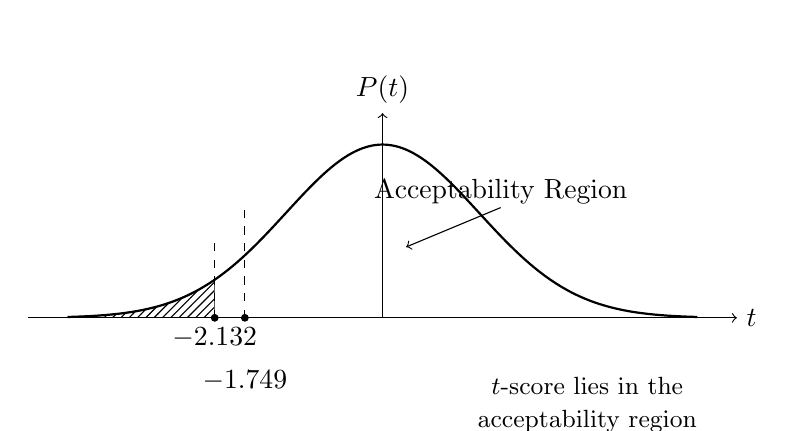
\begin{tikzpicture}[scale=1.0]
  % normal-ish bell curve
  \draw[->] (-4.5,0) -- (4.5,0) node[right] {$t$};
  \draw[->] (0,0) -- (0,2.6) node[above] {$P(t)$};
  \draw[domain=-4:4, smooth, variable=\x, samples=100, thick]
       plot ({\x},{2.2*exp(-\x*\x/3)});
  % critical value and t-score marks
  \draw[dashed] (-2.132,0) -- (-2.132,1.0);
  \node[below] at (-2.132,0) {$-2.132$};
  \draw[dashed] (-1.749,0) -- (-1.749,1.4);
  \node[below] at (-1.749,-0.55) {$-1.749$};
  \filldraw (-2.132,0) circle (1.2pt);
  \filldraw (-1.749,0) circle (1.2pt);
  % shaded rejection region (left tail beyond -2.132)
  \begin{scope}
    \clip (-4,0) rectangle (-2.132,2.6);
    \draw[domain=-4:-2.132, smooth, variable=\x, samples=50, pattern=north east lines]
         plot ({\x},{2.2*exp(-\x*\x/3)}) -- (-2.132,0) -- (-4,0) -- cycle;
  \end{scope}
  \node at (1.5,1.6) {Acceptability Region};
  \draw[->] (1.5,1.4) -- (0.3,0.9);
  \node[align=center] at (2.6,-1.1) {\small $t$-score lies in the\\\small acceptability region};
\end{tikzpicture}
\end{center}
\mk{1 mark}

%================================================================
\section{Question 3 -- One-sample $Z$-test: weight change in cancer patients (Marks: 2+6 = 8)}
\begin{question}{Q3}
A large sample of 100 cancer patients is randomly selected to find the weight change in 2 weeks from the intake of a food supplement. The mean weight change was $+1.2$ kg, and std.\ dev.\ was 0.8 kg. At the population level, the mean weight change of cancer patients is $-0.5$ kg (in the same time).
\begin{enumerate}[label=\roman*)]
\item State hypotheses to evaluate if weight change of this sample is \emph{different} from the reference.
\item Evaluate your hypothesis at a confidence interval of 95\%.
\end{enumerate}
\end{question}

\soln

\subsection*{i) Hypothesis}
\[
H_0: \mu = \mu_0\ (-0.5)
\]
\[
H_A: \mu \neq \mu_0\ (-0.5) \mk{2 marks}
\]

\begin{tcolorbox}[colback=gray!5, colframe=gray!60, title=Note (from original marking scheme)]
Mentioning any value other than $-0.5$ leads to a $-\frac{1}{2}$ mark deduction. Not mentioning any value is okay.
\end{tcolorbox}

\subsection*{ii) Sample statistics and test}
\[
n=100\ (\ge30), \qquad \text{mean } \bar{x}=1.2\ \text{kg}, \qquad \text{std.\ dev. } s=0.8\ \text{kg}, \qquad \text{var } s^2 = 0.64\ \text{kg}^2
\]
\[
SE = \frac{s}{\sqrt{n}} = \frac{0.8}{\sqrt{100}} = \frac{0.8}{10} = 0.08 \mk{2 marks}
\]

We wish to evaluate whether this sample is different from the population, reference value $\mu_0=-0.5$ kg. Since the sample is large ($n\ge30$), we will use the \textbf{$Z$-test}.

\[
Z_{score} = \frac{\bar{x}-\mu_0}{SE} = \frac{1.2-(-0.5)}{0.08}
\]
\[
\boxed{Z_{score} = 21.25} \mk{2 marks}
\]

The CI at 95\%, i.e., $\alpha=0.05$ for a two-tailed $Z$-test:
\[
Z_{\alpha/2} = 1.96 \mk{1 mark}
\]

Now, $|21.25| > 1.96$. \textbf{We reject $H_0$} (or accept $H_A$). \mk{1 mark}

%================================================================
\section{Question 4 -- Two-sample $t$-test (pooled variance): legume protein content (Marks: 2+5+1 = 8)}
\begin{question}{Q4}
A nutritionist is interested in comparing the protein content (arb.\ units) in two legume species. She tested two random samples, whose statistics are reported below:

\begin{center}
\begin{tabular}{lcc}
\toprule
 & Legume-1 & Legume-2 \\
\midrule
Sample size & 8 & 8 \\
Mean & 18.2 & 14.4 \\
Variance & 4.0 & 3.2 \\
\bottomrule
\end{tabular}
\end{center}

She supposes that at the population level, there is no difference in their mean protein content.
\begin{enumerate}[label=\roman*)]
\item State hypotheses for the nutritionist. State the most appropriate test in this case.
\item Evaluate the hypothesis based on the data provided at $\alpha=0.05$.
\item Schematically depict the relevant distribution, marking the ``acceptability region''.
\end{enumerate}
\end{question}

\soln

\textbf{Given:}
\[
n_1=n_2=8, \qquad \bar{x}_1=18.2,\ s_1^2=4.0, \qquad \bar{x}_2=14.4,\ s_2^2=3.2
\]

\subsection*{i) Hypothesis and test choice}
\[
H_0: \mu_1=\mu_2
\]
\[
H_1: \mu_1\neq\mu_2 \mk{1 mark}
\]

\textbf{Most Appropriate Test: Two-Sample $t$-test with pooled variance} \mk{1 mark}
(appropriate since both sample sizes are small and equal, and the two sample variances are reasonably similar, so a pooled-variance approach is justified.)

\subsection*{ii) Evaluation}

\textbf{Pooled variance:}
\[
Var = \frac{(n_1-1)s_1^2+(n_2-1)s_2^2}{n_1+n_2-2}
\]
\[
= \frac{7\times4.0+7\times3.2}{14} = 3.6 \mk{1 mark}
\]

\textbf{Standard Error:}
\[
SE = s_p\sqrt{\frac{1}{n_1}+\frac{1}{n_2}}
\]
\[
= 1.897\sqrt{0.28} = 0.9487 \mk{1 mark}
\]

\textbf{$t$-score:}
\[
t = \frac{\bar{x}_1-\bar{x}_2}{SE} = \frac{18.2-14.4}{0.9487}
\]
\[
\boxed{t = 4.01} \mk{1 mark}
\]

\textbf{Degrees of freedom:}
\[
\nu = n_1+n_2-2 = 14 \mk{1 mark}
\]

\[
\alpha=0.05
\]
\[
t_{critical} = t_{\alpha/2,\,\nu} = t_{0.025,\,14} = 2.145
\]

Since $t_{score} > t_{critical}$, \textbf{Reject $H_0$.} \mk{1 mark}

\subsection*{iii) Schematic of the distribution}

\begin{center}
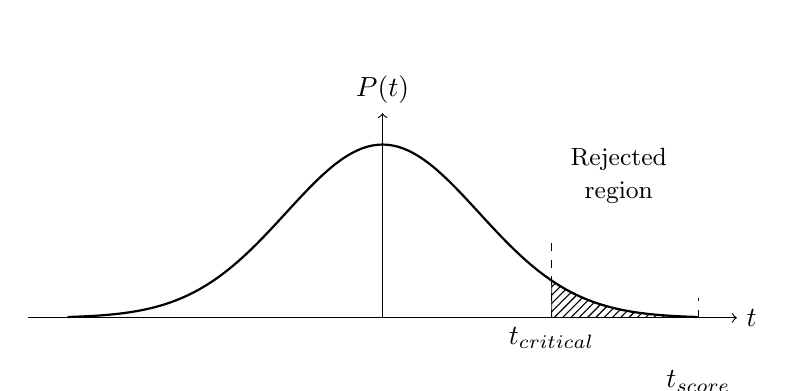
\begin{tikzpicture}[scale=1.0]
  \draw[->] (-4.5,0) -- (4.5,0) node[right] {$t$};
  \draw[->] (0,0) -- (0,2.6) node[above] {$P(t)$};
  \draw[domain=-4:4, smooth, variable=\x, samples=100, thick]
       plot ({\x},{2.2*exp(-\x*\x/3)});
  \draw[dashed] (2.145,0) -- (2.145,1.0);
  \node[below] at (2.145,0) {$t_{critical}$};
  \draw[dashed] (4.01,0) -- (4.01,0.25);
  \node[below] at (4.01,-0.55) {$t_{score}$};
  \begin{scope}
    \clip (2.145,0) rectangle (4.4,2.6);
    \draw[domain=2.145:4, smooth, variable=\x, samples=50, pattern=north east lines]
         plot ({\x},{2.2*exp(-\x*\x/3)}) -- (4,0) -- (2.145,0) -- cycle;
  \end{scope}
  \node[align=center] at (3.0,1.8) {\small Rejected\\\small region};
\end{tikzpicture}
\end{center}
\mk{1 mark}

%================================================================
\section{Formula Sheet}
\begin{tcolorbox}[colback=qcolor!5, colframe=qcolor, title=Formulae provided with the paper]

\[
Z = \frac{\bar{X}-\mu}{\sigma_{\bar{X}}}
\]

\[
Z_{score} = \frac{[\bar{X}_1-\bar{X}_2]-[\mu_1-\mu_2]}{\sqrt{\dfrac{\sigma_1^2}{n_1}+\dfrac{\sigma_2^2}{n_2}}}
\]

\[
t_{score} = \frac{[\bar{X}_1-\bar{X}_2]-[D_0]}{\sqrt{s^2\left(\dfrac{1}{n_1}+\dfrac{1}{n_2}\right)}}
\]

\[
\text{approx.}\ \nu \approx \frac{\left[\dfrac{s_1^2}{n_1}+\dfrac{s_2^2}{n_2}\right]^2}{\dfrac{\left(s_1^2/n_1\right)^2}{n_1-1}+\dfrac{\left(s_2^2/n_2\right)^2}{n_2-1}}
\]

\[
Var = \frac{(n_1-1)s_1^2+(n_2-1)s_2^2}{(n_1+n_2-2)}
\]

\[
t_{score} = \frac{[\bar{X}_1-\bar{X}_2]-[D_0]}{\sqrt{\left(\dfrac{s_1^2}{n_1}+\dfrac{s_2^2}{n_2}\right)}}
\]

\end{tcolorbox}

\end{document}
